\chapter{Specification \& Design}

This section describes a high-level design of the system to be implemented. As mentioned in the Requirements section, this will also be the first version of the design documentation. It will be added on to in the future.

\begin{figure}[h]
\centering
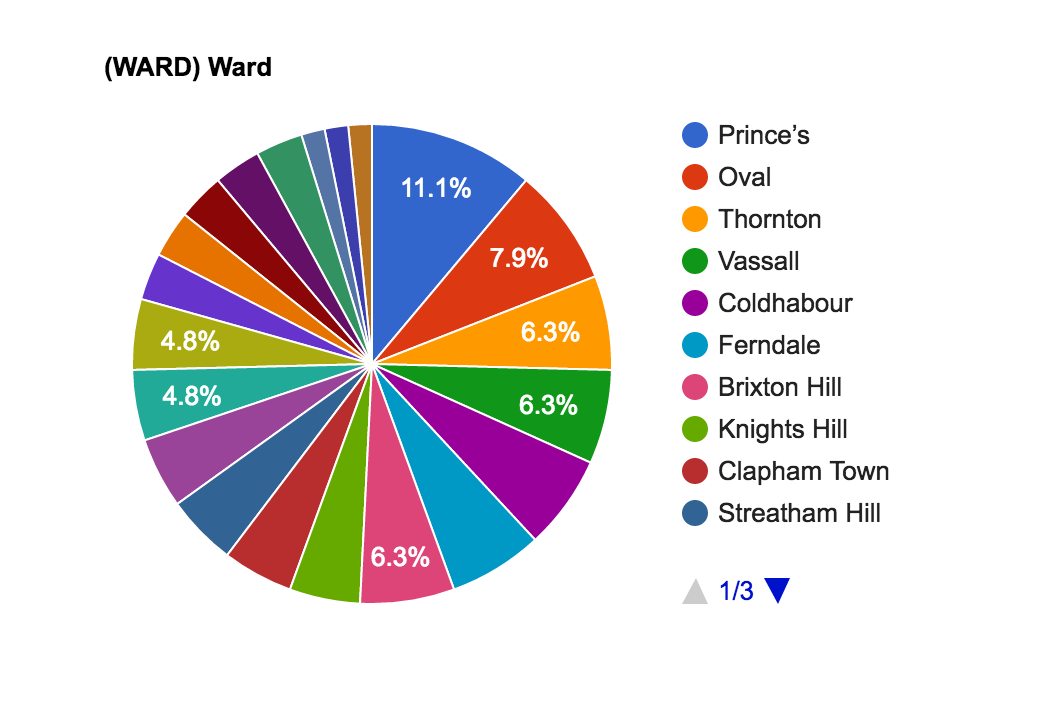
\includegraphics[scale=0.5]{piechart}
\caption{Pie chart visualization}
\end{figure}

\section{System architecture}
Due to the iterative nature of implementation, the architecture chosen will make it easy to add more components and even more data sources. The system will follow the three-layer architecture. The data layer will consist of the survey data and cluster criteria, parameters (based on the 5 clustering factors) for clusters set by the user. The logic layer will consist of creating clusters and extracting clusters from survey data. The presentation layer includes the form to create clusters and the navigation between clusters and visualization of cluster data.

\section{User interface}
The system’s main goal is to present data and let the user interact with the user in an effective way. Thus the design of the user interface is integral to the success of the system.

The cluster creation UI will enable the user to name and enter the parameters for a cluster. The choices for the parameters will be constrained to the fields in the survey and the field’s answers.

To enable the easily navigate between each cluster, there will be a navigation pane in the form of tabs for each cluster. Once a tab is selected, the graphs of data listed in section (data visualization) will be displayed. To enable comparison between data on each cluster, inspired by (kent and medway), each graph will be shown as indexed horizontal bar charts (figure). This will visualize the comparison of the values of the cluster to average value for that field in the whole population.
